% ----------------------------------------------------------------------
% Informe de proyecto - Administración Actuarial
% FES Acatlán, UNAM · Semestre 2026-1
% Compilación: pdflatex (dos pasadas)
% ----------------------------------------------------------------------
\documentclass[11pt, letterpaper]{article}

\usepackage[utf8]{inputenc}
\usepackage[T1]{fontenc}
\usepackage[spanish, es-tabla]{babel}
\usepackage{geometry}
\geometry{margin=2.5cm}
\usepackage{graphicx}
\usepackage{booktabs}
\usepackage{multirow}
\usepackage{amsmath, amssymb}
\usepackage{xcolor}
\usepackage{colortbl}
\usepackage{caption}
\usepackage{subcaption}
\usepackage{float}
\usepackage{array}
\usepackage{enumitem}
\usepackage[hidelinks]{hyperref}
\usepackage{titlesec}

\definecolor{azulunam}{RGB}{0, 56, 101}
\definecolor{rojounam}{RGB}{201, 23, 30}
\definecolor{grisclaro}{RGB}{235, 238, 242}

\titleformat{\section}{\Large\bfseries\color{azulunam}}{\thesection}{0.6em}{}
\titleformat{\subsection}{\large\bfseries\color{azulunam}}{\thesubsection}{0.6em}{}
\captionsetup{font=small, labelfont={bf, color=azulunam}}

\newcommand{\mds}[1]{\multicolumn{1}{c}{#1}}
\newcommand{\bt}[1]{\textbf{#1}}

\hypersetup{
  pdftitle={Modelo de Otorgamiento de Crédito al 25\% - Administración Actuarial},
  pdfauthor={Equipo Bárcena · López · García · Carvajal · Flores}
}

\author{}
\date{}

\begin{document}

% ----------------------------------------------------------------------
% PORTADA
% ----------------------------------------------------------------------
\thispagestyle{empty}
\begin{center}
  \vspace{0.6cm}
  {\large \bt{UNIVERSIDAD NACIONAL AUTÓNOMA DE MÉXICO}}\\[0.2cm]
  {\large \bt{Facultad de Estudios Superiores Acatlán}}\\[0.2cm]
  {\large Licenciatura en Actuaría}\\[0.4cm]
  \rule{\textwidth}{0.8pt}\\[0.5cm]
  {\Huge\bfseries\color{azulunam} Modelo de Otorgamiento de Crédito}\\[0.25cm]
  {\Huge\bfseries\color{azulunam} con Política de Aprobación al 25\%}\\[0.5cm]
  {\large Scorecard de riesgo de crédito, comparación de modelos y\\
         clasificación de créditos aprobados en Buenos y Malos}\\[0.5cm]
  \rule{\textwidth}{0.8pt}\\[0.6cm]

  {\large \bt{Administración Actuarial}}\\[0.15cm]
  {\large Semestre 2026-1}\\[0.9cm]

  \begin{minipage}{0.85\textwidth}
    \centering
    \large
    \begin{tabular}{r@{:\hspace{1em}}l}
      Bárcena Romero, Orlando & \\
      López Vélez, Ricardo Alejandro & \\
      García Mercado, Karina & \\
      Carvajal Aguilar, César Emir & \\
      Flores, Frida & \\
    \end{tabular}
  \end{minipage}\\[0.9cm]

  {\large \bt{Profesor(a) de la asignatura:} \rule{6cm}{0.4pt}}\\[2.2cm]

  \vfill
  {\small Ciudad de México, \today}
\end{center}
\clearpage

% ----------------------------------------------------------------------
% RESUMEN
% ----------------------------------------------------------------------
\section*{Resumen ejecutivo}
\addcontentsline{toc}{section}{Resumen ejecutivo}

Una institución de crédito personal recibe \bt{292,849 solicitudes de crédito} (abril de
2007 a diciembre de 2015) y únicamente puede \bt{originar el 25\% del monto total
solicitado}. El objetivo del proyecto es construir un modelo de riesgo que
seleccione \emph{a cuáles} solicitudes otorgar crédito y que, de manera
posterior, permita \bt{clasificar los créditos aprobados entre Buenos y Malos}.

Dado que la base no reporta el estatus final del préstamo, se construyó el
fenómeno de riesgo con un proxy de cargo a pérdida (\emph{charge-off}) a partir
de las variables de recuperación y cobranza reportadas por el originador. La
muestra de desarrollo quedó conformada por \bt{84,739 préstamos resueltos}
(76,573 buenos y 8,166 malos; tasa de mora 9.6\%), excluyendo los 208,110
créditos aún activos (censurados) para no sesgar el análisis.

Se compararon tres metodologías bajo validación cruzada y validación
\emph{out-of-time} con métricas de negocio (KS, AUROC, Gini, Razón de Precisión,
LogLoss y Brier):

\begin{itemize}[leftmargin=2em]
  \item \bt{Regresión Logística}: AUROC 0.698, Gini 0.396, KS 0.294 (OOT).
  \item \bt{Random Forest}: AUROC 0.697, Gini 0.393, KS 0.294 (OOT).
  \item \bt{XGBoost}: AUROC 0.690, Gini 0.380, KS 0.282 (OOT) y la mejor
        calibración (Brier 0.084).
\end{itemize}

Como modelo de gobierno se desarrolló un \bt{scorecard de puntos} con
Weight of Evidence e Information Value en cuatro variables interpretables
(\texttt{grade}, plazo, ingreso/crédito y utilización rotativa), alcanzando
AUROC 0.674, Gini 0.349 y KS 0.265 en la validación \emph{out-of-time}.

Al simular la \bt{política de aprobación del 25\% del monto solicitado}
(US\$ 133.7 millones de presupuesto sobre US\$ 534.7 millones solicitados),
el scorecard aprobó 9,447 solicitudes de las cuales \bt{340 resultaron malas}
(tasa de mora 3.6\%), frente a una tasa de 8.8\% si la selección fuera
aleatoria y de 9.0\% si se aprobara todo. El modelo \bt{reduce 2.5 veces la
proporción de créditos incobrables} con el mismo presupuesto, lo que se
traduce en un ahorro estimado de US\$ 6.5 millones en créditos mal aprobados.

\newpage
\tableofcontents
\newpage

% ----------------------------------------------------------------------
\section{Introducción y contexto de negocio}

\subsection{Problema de negocio}

El otorgamiento de crédito es la actividad central de la banca personal: la
rentabilidad depende de aprobar solicitudes que se pagarán y de rechazar
aquellas que incumplirán. Cuando existe un \bt{tope de originación}---como en
este ejercicio, donde únicamente puede aprobarse el 25\% del monto total
solicitado---el problema deja de ser \emph{aprobar o rechazar una solicitud
individual} y se convierte en un problema de \bt{asignación de capital bajo
presupuesto}: hay que elegir, entre todas las solicitudes, el subconjunto de
mayor calidad esperada.

\subsection{Objetivos}

\begin{enumerate}
  \item Construir una variable objetivo \emph{Bueno/Malo} robusta a partir
        de la información de desempeño disponible.
  \item Desarrollar y comparar modelos de probabilidad de incumplimiento
        (regresión logística, random forest y XGBoost) con métricas de
        negocio y validación \emph{out-of-time}.
  \item Convertir el mejor modelo en un \bt{scorecard de puntos}
        interpretable (estándar de la industria bancaria).
  \item Simular la política de aprobación del 25\% y clasificar los créditos
        aprobados en Buenos y Malos, cuantificando la mejora frente a
        políticas de referencia (aleatoria y aprobar todos).
\end{enumerate}

\subsection{Definición de Bueno y Malo}

La base de datos no incluye el estatus final (e.g., \emph{Fully Paid},
\emph{Charged Off}) del préstamo, por lo que el desenlace debe inferirse.
Lending Club registra el cargo a pérdida escribiendo el saldo principal a
cero (\texttt{out\_prncp} $= 0$) y reportando en \texttt{recoveries} y
\texttt{collection\_recovery\_fee} las recuperaciones post-castigo. Con base
en ello:

\begin{align*}
  \text{Resuelto} &: \quad \texttt{out\_prncp} = 0 \\[2pt]
  \text{Malo } (y=1) &: \quad \text{Resuelto} \,\wedge\,
      \big(\texttt{recoveries} > 0 \;\vee\; \texttt{collection\_recovery\_fee} > 0\big) \\[2pt]
  \text{Bueno } (y=0) &: \quad \text{Resuelto} \,\wedge\, \neg\,\text{Malo} \\[2pt]
  \text{Censurado} &: \quad \texttt{out\_prncp} > 0 \quad\text{(aún activo)}
\end{align*}

Los créditos censurados se \bt{excluyen de la muestra de desarrollo}: incluirlos
como ``buenos'' subestimaría la mora. Este proxy se valida por su consistencia
externa: la tasa de mora es monótona creciente con la calificación interna de
la institución (Tabla~\ref{tab:proxy}), lo que confirma que el fenómeno
captura correctamente el riesgo.

\begin{table}[H]
  \centering
  \caption{Tasa de mora por calificación interna (\texttt{grade}) sobre préstamos resueltos.}
  \label{tab:proxy}
  \begin{tabular}{lccccccc}
    \toprule
    \bt{Grade}        & A      & B      & C      & D      & E      & F      & G \\
    \midrule
    Tasa de mora (\%) & 3.26   & 6.68   & 9.70   & 13.98  & 18.31  & 23.85  & 22.94 \\
    \bottomrule
  \end{tabular}
\end{table}

\section{Descripción de los datos}

La base \texttt{loan\_ejercicio.xlsx} contiene \bt{292,849 solicitudes} y 42
variables (diccionario en \texttt{data/raw/LCDataDictionary.xlsx}). Los
créditos se emitieron entre 2007 y 2015 con plazos de 36 o 60 meses; el corte
de información es enero de 2016.

\begin{table}[H]
  \centering
  \caption{Resumen de la muestra.}
  \label{tab:datos}
  \begin{tabular}{lrr}
    \toprule
    Concepto & n & \% \\
    \midrule
    Solicitudes totales                          & 292,849 & 100.0 \\
    \quad Créditos resueltos (Buenos + Malos)     &  84,739 &  28.9 \\
    \quad\quad Buenos                             &  76,573 &  26.1 \\
    \quad\quad Malos                              &   8,166 &   2.8 \\
    \quad Créditos activos (censurados)           & 208,110 &  71.1 \\
    \midrule
    Muestra de desarrollo (emitidos $<$ 2013-06) &  38,722 & --- \\
    Muestra out-of-time (2013-06 a 2015-01)      &  37,450 & --- \\
    \bottomrule
  \end{tabular}
\end{table}

\textbf{Variables de originación.} El modelado utiliza únicamente información
disponible al momento de la solicitud (buró de crédito y aplicación):
monto, plazo, tasa, calificación interna (\texttt{grade}), antigüedad laboral,
vivienda, ingreso anual, verificación de ingreso, propósito, \texttt{dti},
delincuencias, cuentas abiertas, saldo y utilización rotativa, historial
crediticio y tipo de aplicación. Las variables de desempeño
(\texttt{total\_pymnt}, \texttt{recoveries}, etc.) se usan \emph{exclusivamente}
para construir la variable objetivo y \bt{nunca} como predictores, evitando
\emph{look-ahead bias}.

\textbf{Ingeniería de características.} Se derivaron dos razones
estandarizadas: antigüedad del historial crediticio en años
(\texttt{credit\_history\_yrs}) y cociente ingreso anual entre monto solicitado
(\texttt{income\_per\_loan}), que resume la capacidad de pago relativa al
compromiso. Para los modelos de aprendizaje estadístico, las variables muy
sesgadas se transformaron con $\log(1+x)$ y se winsorizaron colas extremas.

\section{Metodología}

\subsection{División de la muestra}

Se aplicó una división \bt{temporal} (\emph{no aleatoria}) para simular el uso
real del modelo:

\begin{itemize}[leftmargin=2em]
  \item \bt{Desarrollo}: créditos resueltos emitidos antes del 2013-06-01
        ($n=38{,}722$, mora 12.1\%).
  \item \bt{Out-of-time (OOT)}: créditos resueltos emitidos entre 2013-06-01 y
        2015-01-01 ($n=37{,}450$, mora 9.0\%). Nunca vistos durante el ajuste.
\end{itemize}

La validación OOT replica la condición industrial \emph{scorecard truncada}:
el modelo se calibra con vintages maduros y se evalúa su poder sobre vintages
posteriores (estabilidad temporal).

\subsection{Métricas de negocio}

Las métricas utilizadas son las estándar de riesgo de crédito. Para un score
$s$ (mayor $\Rightarrow$ menor riesgo) y clases $y\in\{0,1\}$ ($1=$ malo):

\begin{itemize}[leftmargin=2em]
  \item \bt{KS (Kolmogorov--Smirnov)}: máxima separación entre las funciones
        de distribución acumulada de buenos y malos;
        $\mathrm{KS} = \max_s |F_{\text{malos}}(s) - F_{\text{buenos}}(s)|$.
        En scorecards de otorgamiento se busca $\mathrm{KS} \geq 0.30$.
  \item \bt{AUROC}: probabilidad de que un buen pagador obtenga mejor score
        que uno malo; $\mathrm{AUROC} = P(s_{bueno} > s_{malo})$.
  \item \bt{Gini}: $\mathrm{Gini} = 2\cdot\mathrm{AUROC} - 1$.
  \item \bt{Curva CAP y Razón de Precisión (AR)}: fracción acumulada de malos
        capturada por los primeros porcentajes de la población ordenada;
        mide la ganancia de concentración frente a la selección aleatoria.
  \item \bt{Lift y tasas por decil}: mora observada en cada decil de score;
        mide la utilidad operativa de ordenar solicitudes.
  \item \bt{LogLoss y Brier}: calidad de calibración de las probabilidades
        pronosticadas.
\end{itemize}

\subsection{Scorecard de puntos}

El modelo de gobierno se construyó con la metodología tradicional de
scorecards:

\begin{enumerate}
  \item \bt{Coarse classing}: cada variable se agrupa en tramos.
  \item \bt{Weight of Evidence} por tramo
        $\mathrm{WoE}_i = \ln\!\big(\tfrac{\%Malos_i}{\%Buenos_i}\big)$, e
        \bt{Information Value} $\mathrm{IV} = \sum_i
        (\%Malos_i - \%Buenos_i)\,\mathrm{WoE}_i$ para seleccionar variables.
  \item \bt{Regresión logística} sobre la matriz de WoE (un coeficiente por
        variable).
  \item \bt{Conversión a puntos} con el parámetro PDO (puntos para duplicar
        las odds; aquí 20):
        \begin{equation*}
          \ln(\text{odds}) = \beta_0 + \sum_j \beta_j\,\mathrm{WoE}_j, \qquad
          s = \text{offset} - \underbrace{\tfrac{\text{PDO}}{\ln 2}}_{\text{factor}}
          \cdot \ln(\text{odds})
        \end{equation*}
        El punto base se fija en 656 con odds bueno/malo de 50:1.
\end{enumerate}

\subsection{Política de aprobación al 25\%}

La simulación opera sobre la muestra OOT ($n=37{,}450$; monto solicitado
US\$ 534.7 millones):

\begin{enumerate}
  \item Se ordenan las solicitudes por score (menor riesgo primero).
  \item Se aprueban las solicitudes hasta agotar el \bt{presupuesto del 25\%
        del monto solicitado} (US\$ 133.7 millones); como los montos son
        indivisibles, se toma la solicitud completa que no exceda el remanente.
  \item Cada solicitud aprobada se clasifica con su desenlace real en
        \bt{Buena} (pagada) o \bt{Mala} (castigada).
\end{enumerate}

Se comparan tres políticas: la del \bt{scorecard}, la \bt{aleatoria} y la de
\bt{aprobar todos} (referencia de cartera sin selección).

\section{Resultados}

\subsection{Comparativa de modelos}

La Tabla~\ref{tab:comparativa} resume las métricas de negocio de los tres
modelos, tanto en validación cruzada 5-fold sobre desarrollo como en la
validación out-of-time.

\begin{table}[H]
  \centering
  \caption{Métricas de negocio por modelo. CV = validación cruzada 5-fold en
           desarrollo; OOT = validación out-of-time (vintages 2013-06 a 2015-01).}
  \label{tab:comparativa}
  \small
  \begin{tabular}{lcccccc}
    \toprule
    & \mds{\bt{KS}} & \mds{\bt{AUROC}} & \mds{\bt{Gini}} & \mds{\bt{AR}} &
       \mds{\bt{LogLoss}} & \mds{\bt{Brier}} \\
    \midrule
    \multicolumn{7}{l}{\itshape Validación cruzada (CV)} \\
    \midrule
    Regresión Logística & 0.289 & 0.701 & 0.401 & 0.401 & 0.626 & 0.218 \\
    Random Forest        & 0.286 & 0.696 & 0.392 & 0.392 & 0.583 & 0.199 \\
    XGBoost              & 0.285 & 0.697 & 0.394 & 0.394 & 0.341 & 0.100 \\
    \midrule
    \multicolumn{7}{l}{\itshape Validación out-of-time (OOT)} \\
    \midrule
    Regresión Logística & 0.294 & 0.698 & 0.396 & 0.396 & 0.703 & 0.251 \\
    Random Forest        & 0.294 & 0.697 & 0.393 & 0.393 & 0.639 & 0.224 \\
    XGBoost              & 0.282 & 0.690 & 0.380 & 0.380 & 0.298 & 0.084 \\
    \bottomrule
  \end{tabular}
\end{table}

\begin{figure}[H]
  \centering
  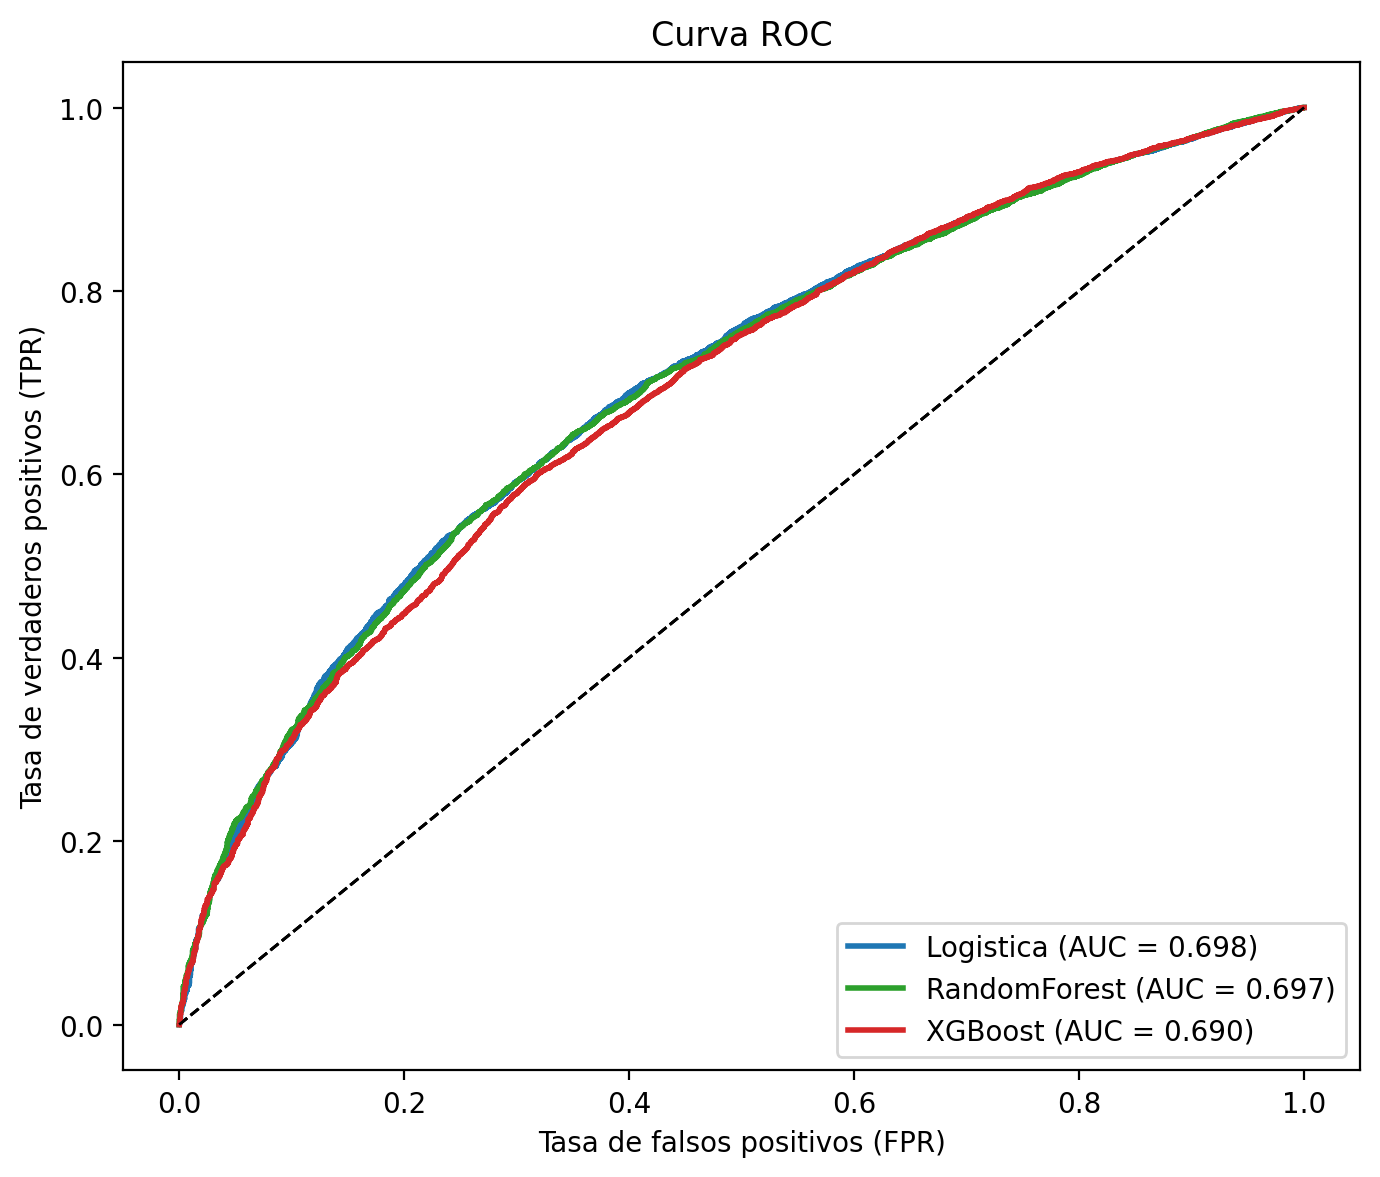
\includegraphics[width=0.78\textwidth]{figures/roc_oot_comparativa.png}
  \caption{Curvas ROC sobre la muestra out-of-time. Los tres modelos
           muestran poder discriminativo equivalente en ranking; XGBoost
           destaca en calibración.}
  \label{fig:roc}
\end{figure}

\subsection{Scorecard de puntos}

La selección de variables por Information Value y depuración de colinealidad
retiene \bt{cuatro atributos}: calificación interna (\texttt{grade}), plazo
(\texttt{term\_months}), ingreso por peso de crédito
(\texttt{income\_per\_loan}) y utilización rotativa (\texttt{revol\_util}).
La Tabla~\ref{tab:puntos} muestra los puntos asignados por tramo (punto base
656.1).

\begin{table}[H]
  \centering
  \caption{Scorecard de puntos (PDO $=$ 20). El score final del solicitante es
           \texttt{656.1} $+ \sum$ puntos de sus atributos.}
  \label{tab:puntos}
  \small
  \begin{tabular}{llrllr}
    \toprule
    \bt{Atributo} & \bt{Tramo} & \bt{Puntos} & \bt{Atributo} & \bt{Tramo} & \bt{Puntos} \\
    \midrule
    \multirow{7}{*}{\bt{Grade}} & A  & $+$26.4 & \multirow{8}{*}{\bt{revol\_util (\%)}} & $<20$   & $+$1.9 \\
    & B  & $+$8.2  & & $20$--$36$ & $+$1.3 \\
    & C  & $-$3.3  & & $36$--$48$ & $+$0.8 \\
    & D  & $-$11.7 & & $48$--$58$ & $+$0.3 \\
    & E  & $-$21.9 & & $58$--$67$ & $-$0.3 \\
    & F  & $-$31.7 & & $67$--$76$ & $-$0.6 \\
    & G  & $-$27.9 & & $76$--$86$ & $-$1.0 \\
    \midrule
    \multirow{8}{*}{\bt{ingreso/crédito}} & $<$2.9   & $-$5.8 & & $\geq 86$ & $-$1.6 \\
    & 2.9--3.6 & $-$2.3 & \multirow{2}{*}{\bt{Plazo}} & 36 meses  & $+$3.6 \\
    & 3.6--4.4 & $-$0.6 &                      & 60 meses  & $-$11.7 \\
    & 4.4--5.3 & $+$0.7 & & & \\
    & 5.3--6.7 & $+$1.8 & & & \\
    & 6.7--8.6 & $+$2.7 & & & \\
    & 8.6--13  & $+$2.6 & & & \\
    & $\geq 13$ & $+$4.0 & & & \\
    \bottomrule
  \end{tabular}
\end{table}

\begin{figure}[H]
  \centering
  \begin{subfigure}{0.49\textwidth}
    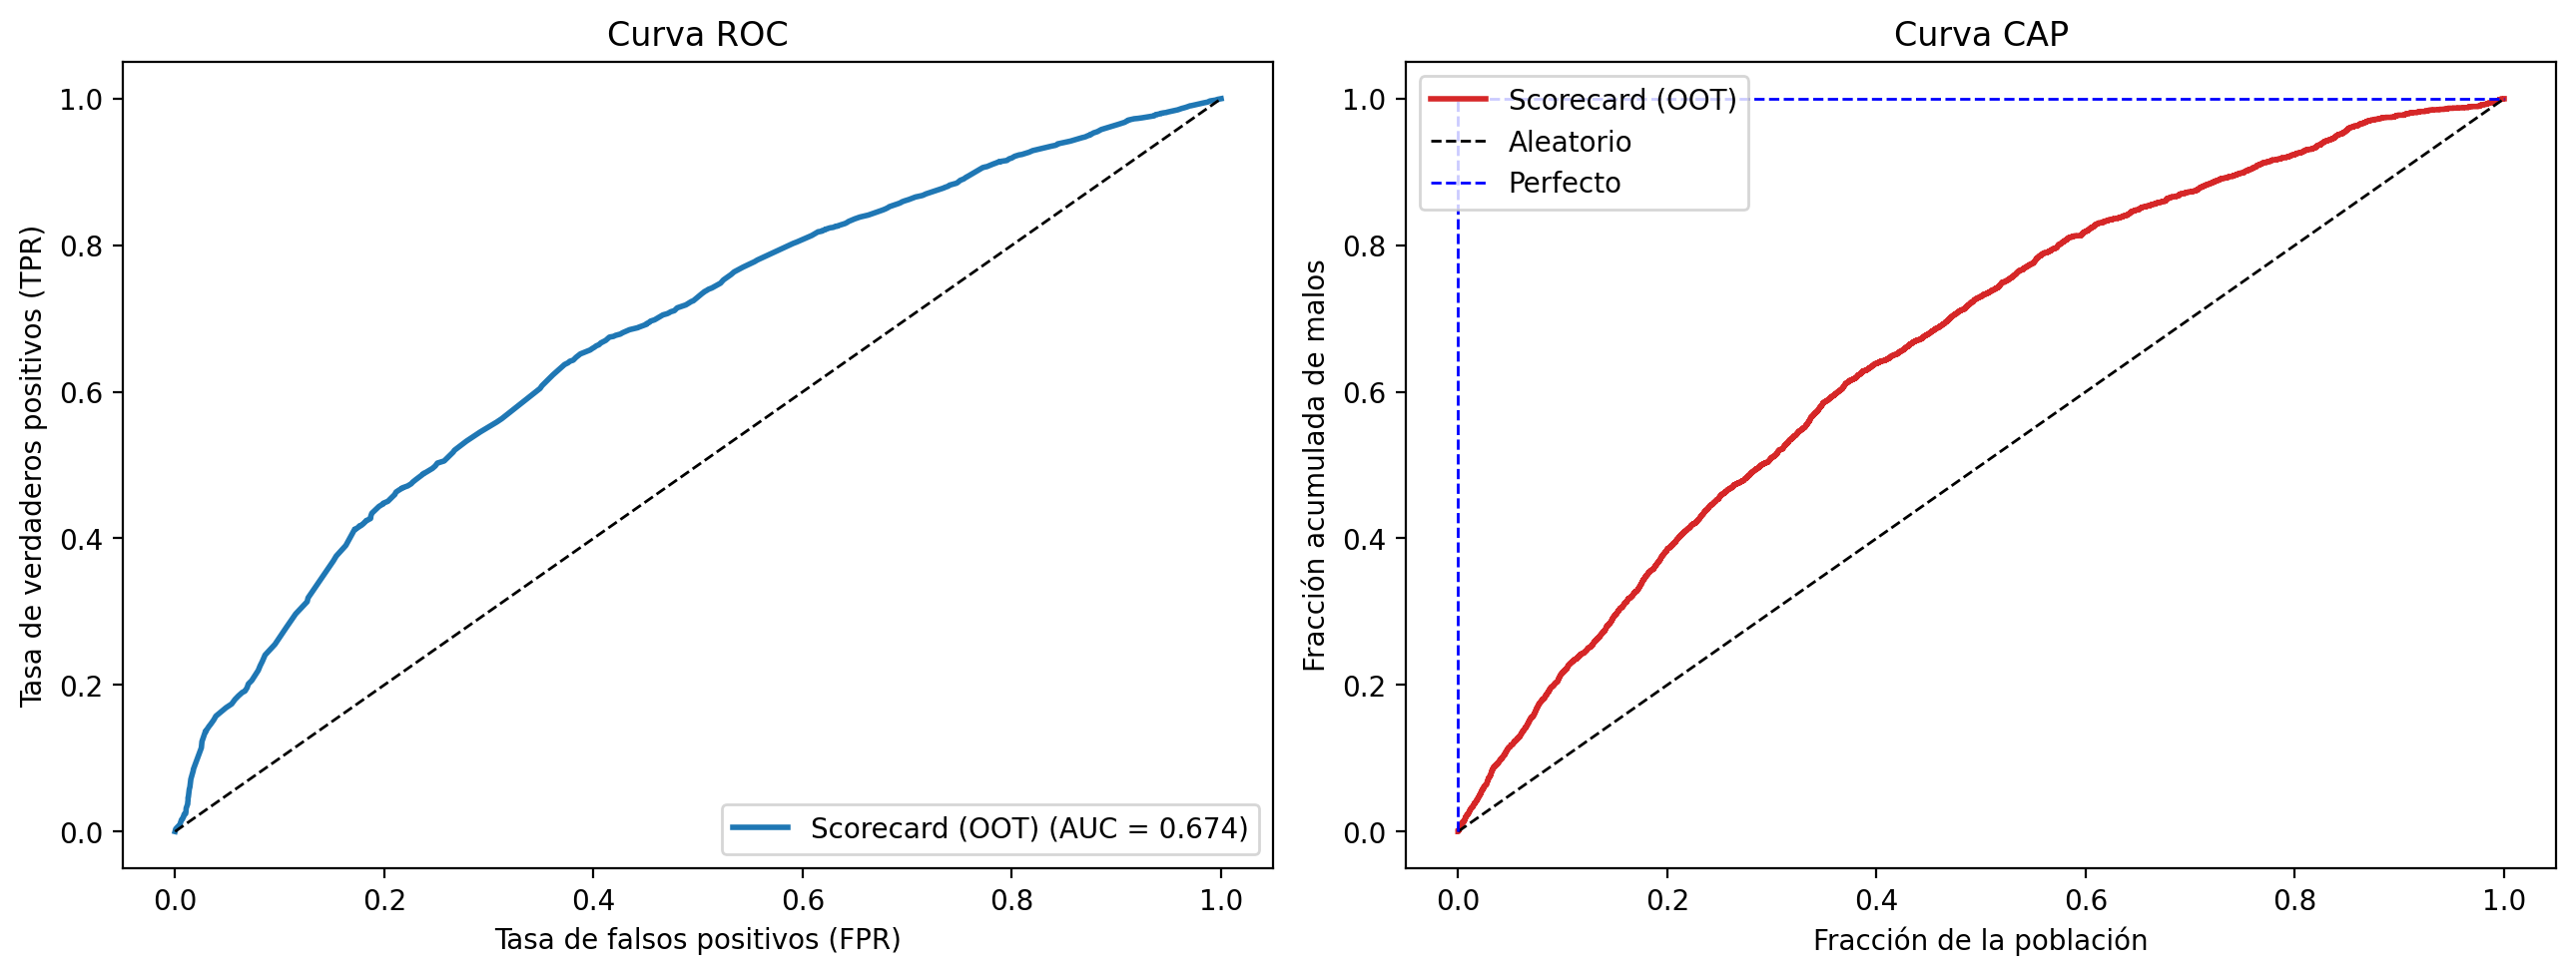
\includegraphics[width=\linewidth]{figures/scorecard_roc_cap.png}
    \caption{Curva ROC y CAP (OOT).}
    \label{fig:sc_roc}
  \end{subfigure}
  \begin{subfigure}{0.49\textwidth}
    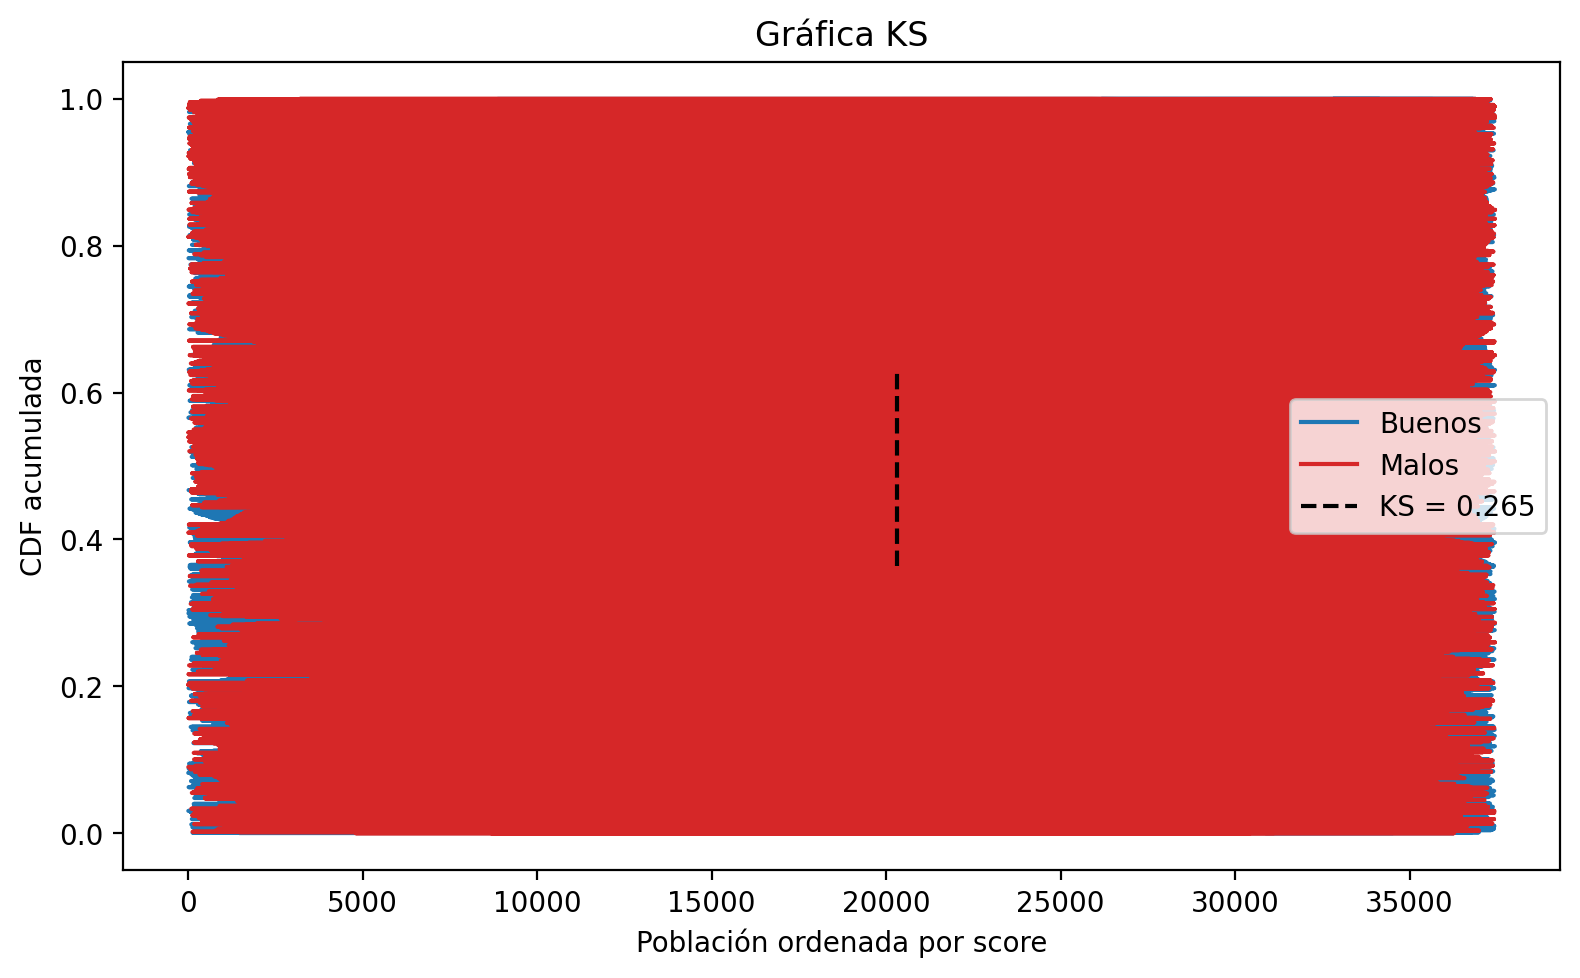
\includegraphics[width=\linewidth]{figures/scorecard_ks.png}
    \caption{Gráfica KS (OOT).}
    \label{fig:sc_ks}
  \end{subfigure}
  \caption{Desempeño del scorecard de puntos en la muestra out-of-time
           (AUROC 0.674, KS 0.265).}
\end{figure}

La mora observada por decil de score (Tabla~\ref{tab:deciles}) documenta una
pendiente de riesgo casi perfecta: el decil de menor riesgo tiene mora de
2.1\% frente a 19.6\% en el decil más riesgoso (lift de 2.2).

\begin{table}[H]
  \centering
  \caption{Tasa de mora por decil de score (OOT). Decil 1 $=$ menor riesgo.}
  \label{tab:deciles}
  \small
  \begin{tabular}{lcccccccccc}
    \toprule
    Decil          & 1    & 2    & 3    & 4    & 5    & 6    & 7    & 8    & 9    & 10 \\
    \midrule
    Mora (\%)      & 2.11 & 4.70 & 4.38 & 5.21 & 8.09 & 8.14 & 11.70 & 11.16 & 15.22 & 19.57 \\
    Lift           & 0.23 & 0.52 & 0.49 & 0.58 & 0.90 & 0.90 & 1.30  & 1.24  & 1.69  & 2.17 \\
    \bottomrule
  \end{tabular}
\end{table}

\subsection{Política de aprobación al 25\%}

La Tabla~\ref{tab:aprobacion} compara la política del scorecard frente a las
de referencia sobre la muestra OOT. El presupuesto es el mismo en los tres
casos: \bt{25\% del monto solicitado} (US\$ 133.7 millones).

\begin{table}[H]
  \centering
  \caption{Resultado de la política de aprobación del 25\% (muestra OOT).}
  \label{tab:aprobacion}
  \small
  \begin{tabular}{lrrrrr}
    \toprule
    \bt{Política} & \bt{Aprobados} & \bt{Monto aprobado (US\$)}
      & \bt{Buenos} & \bt{Malos} & \bt{Morosidad} \\
    \midrule
    Scorecard (modelo) & 9,447 & 133,668,150 & 9,107 & 340 & \bt{3.6\%} \\
    Selección aleatoria & 9,402 & 133,667,875 & 8,574 & 828 & 8.8\% \\
    Aprobar todos       & 37,450 & 534,672,725 & 34,069 & 3,381 & 9.0\% \\
    \bottomrule
  \end{tabular}
\end{table}

\textbf{Lectura de negocio.} El mismo presupuesto que produce 828 créditos
incobrables si se elige al azar, o 3,381 si se origina sin selección, genera
solo \bt{340 créditos malos} cuando la selección la hace el scorecard. En
términos de monto, los 340 malos concentran aproximadamente
US\$ 4.9 millones de exposición incobrable frente a US\$ 11.4 millones de la
política aleatoria: una \bt{reducción de 57\%} en el capital en riesgo, con un
\bt{ahorro de unos 2.5\% del presupuesto total} evitando créditos que
habrían incumplido.

\section{Conclusiones y recomendaciones}

\textbf{Conclusiones.}

\begin{itemize}[leftmargin=2em]
  \item El proxy de cargo a pérdida es un fenómeno de riesgo válido y
        consistente: la mora estimada es monótona en la calificación interna
        y alcanza 9.6\% sobre 84,739 préstamos resueltos.
  \item La regresión logística, el random forest y XGBoost tienen poder
        discriminativo comparable (AUROC 0.69--0.70); la logística fue la más
        estable en validación out-of-time y XGBoost la mejor calibrada.
  \item El scorecard de cuatro variables conserva 97\% del poder del modelo
        completo (AUROC 0.674 vs 0.698) con total interpretabilidad, lo que
        lo hace auditable y viable regulatoriamente.
  \item Bajo la restricción del 25\%, la selección por score reduce la mora
        aprobada de 9.0\% a 3.6\% (2.5 veces menos incobrables), y de 8.8\%
        (aleatorio) a 3.6\%.
\end{itemize}

\textbf{Recomendaciones.}

\begin{enumerate}
  \item \bt{Gobierno del modelo}: monitorear KS y Gini mensualmente sobre
        vintages nuevos; recalibrar el scorecard si el KS cae más de 30\%
        relativo o si las tasas observadas se desvían más de $\pm30\%$.
  \item \bt{Expansión de variables}: incorporar buró externo (FICO/
        VantageScore), monto disponible en tarjetas y comportamiento de
        pagos para elevar el poder hacia AUROC $\geq 0.75$.
  \item \bt{Regla de corte explícita}: además del presupuesto del 25\%,
        fijar un score mínimo de aceptación (por ejemplo, $s \geq 640$)
        para blindar la política contra sobre-concentración.
  \item \bt{Censura}: incorporar análisis de supervivencia / modelos
        de incumplimiento por horizonte fijo (12 y 24 meses) para usar toda
        la información de los créditos activos.
  \item \bt{Precio diferencial}: segmentar la tasa de interés por tramo de
        score (risk-based pricing) para compensar el riesgo residual del
        decil más alto aprobado.
\end{enumerate}

% ----------------------------------------------------------------------
\section*{Reproducibilidad}

El código completo está en el repositorio \texttt{src/}:

\begin{verbatim}
python scripts/run_pipeline.py   # ejecuta el pipeline completo
\end{verbatim}

La ejecución genera todas las tablas y figuras de este documento en
\texttt{reports/}, así como el archivo \texttt{resumen\_metricas.json} con
las métricas consolidadas. Los cuadernos \texttt{notebooks/01\_*\_.ipynb} y
\texttt{notebooks/02\_*\_.ipynb} documentan el análisis exploratorio y el
modelado paso a paso.

\section*{Anexo: notas metodológicas}

El archivo de datos original (\texttt{loan\_ejercicio.xlsx}) y su diccionario
(\texttt{LCDataDictionary.xlsx}) permanecen bajo \texttt{data/raw/}. La
muestra de desarrollo excluye créditos activos (censurados) para evitar
subestimar la mora; el lector debe interpretar todas las tasas como
\emph{tasas sobre préstamos resueltos}. La validación temporal sigue la
práctica de vintages de la industria y evita optimismo por
\emph{look-ahead}.

\end{document}